\documentclass[a4paper,10pt]{article}
\usepackage[utf8]{inputenc}
\usepackage[polish]{babel}
\usepackage{polski}
\usepackage{graphicx}
\usepackage{hyperref}
\hypersetup{colorlinks,citecolor=black,filecolor=black,linkcolor=black,urlcolor=black,pdftex}

\title{\textbf{\begin{LARGE}P.I.W.O. 1.0\end{LARGE}}\\\underline{Projekt Informatyczny} \\ Wilqu \& Others \\\textbf{Instrukcja użytkownika}}

\author{Piotr Wilk \and Piotr Zegar \and Mateusz Tylek \and Mateusz Kocąb \and Wojciech Zbiegieł \and Sławomir Librant \and  Marek Prząda}
\begin{document}
\maketitle
\begin{figure}[h]
 \centering

\includegraphics{logo}
\begin{center}
\begin{center}

\end{center}

 % logo.eps: 0x0 pixel, 300dpi, 0.00x0.00 cm, bb=0 0 160 154
\end{center}

\end{figure}
\newpage
\tableofcontents
\newpage

\section{Wstęp}
P.I.W.O 1.0 jest silnikiem napisanym z myślą o cyfrowym przetważaniu obrazów aczkolwiek dzięki dośc rozbudowanej obsłudze pluginów można nim przetważać dowolne dane. W programie cykl operacji jakie mają zostać wykonane na obiekcie definiujemy w postaci bloczków które można ze sobą łączyć.
\section{Wymagania sprzętowe}
Program nie był jeszcze testowany pod względem wymagań sprzętowych aczkolwiek prawdopodbnie będzie działał na każdej maszynie z
zainstalowanym systemem operacyjnym Widnows 2000,XP,Vista.
\section{Interfejs użytkownika}
\begin{figure}[h]
 \centering
 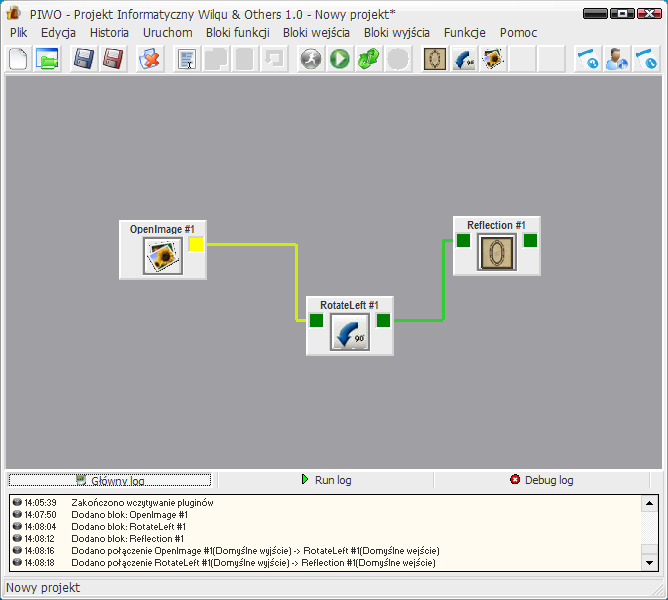
\includegraphics[scale=0.5]{main}
 \caption{Interfejs użytkownika}
 \label{fig:Interface}
\end{figure}
\newpage
Główne okno programu jest podzielone na 4 stefy:
\begin{enumerate}
 \item Menu główne
 \item Toolbar
 \item Strefa projektu
 \item System logów
 \item Pasek status
\end{enumerate}
W tytule okna zawsze zawarta jest nazwa projektu/plik projektu. Gwiazdka na końcu sugeruje iż w projekcie zostały wprowadzone zmiany.
\subsection{Menu główne}
\begin{figure}[h]
 \centering
 
\includegraphics[scale=0.5]{menuglowne}
 \caption{Menu Glowne}
 \label{fig:Interface}
\end{figure}
\subsubsection{Plik}
Menu zawierające opcje pozwalające na zarządzanie projektem.
\begin{description}
\item[Nowy projekt] Zamyka aktualnie otwarty projekt. W przypadku gdy zostały w nim wprowadzone zmiany od czasu ostatniego zapisu lub niebył on zapisywany wcześniej użytkownik zostanie zapytany o zapis projektu lub porzucenie zmian. Tworzy nowy projekt.
\item[Otwórz projekt] Zamyka aktualnie otwarty projekt. W przypadku gdy zostały w nim wprowadzone zmiany od czasu ostatniego zapisu lub niebył on zapisywany wcześniej użytkownik zostanie zapytany o zapis projektu lub porzucenie zmian. Otwiera okno pozwalające na wybranie pliku z którego zostanie wczytany nowy projekt.
\item[Zapisz projekt] Opcja dostępna tylko gdy mamy już otwarty projekt. Jeśli nie był on wcześniej zapisywany to zostanie otwarte okno w którym użytkownik będzie mógł wybrac położenie i nazwę pliku pod którą projekt zostanie zapisany. W przeciwnym wypadku program zapisze projekt używając pliku docelowego który wcześniej już został wybrany.
\item[Zapisz projekt jako] Opcja dostępna tylko gdy mamy już otwarty projekt. Zostanie otwarte okno w którym użytkownik będzie mógł wybrac położenie i nazwę pliku pod którą projekt zostanie zapisany.
\item[Zamknij projekt] Opcja dostępna tylko gdy mamy już otwarty projekt. Zamyka aktualnie otwarty projekt. W przypadku gdy zostały w nim wprowadzone zmiany od czasu ostatniego zapisu lub niebył on zapisywany wcześniej użytkownik zostanie zapytany o zapis projektu lub porzucenie zmian.
\item[Zakończ] Zamyka program, jeśli mamy otwarty projekt i przypadku gdy zostały w nim wprowadzone zmiany od czasu ostatniego zapisu lub niebył on zapisywany wcześniej użytkownik zostanie zapytany o zapis projektu lub porzucenie zmian. 
\end{description}
\subsubsection{Edycja}
\begin{figure}[h]
 \centering
 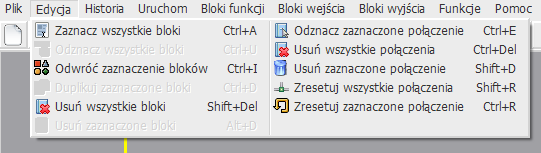
\includegraphics[scale=0.5]{edycja}
 \caption{Edycja}
 \label{fig:edition}
\end{figure}
Wszystkie opcje z tego menu są dostepne tylko i wyłącznie gdy mamy otwarty projekt. Niektóre z nich wymagają aby w projekcie było conajmniej jedno połączenie, blok, lub aby conajmniej jeden blok był zaznaczony lub połączenie.
\begin{description}
\item[Zaznacz wszystkie bloki] Polecenie zaznacza wszystkie bloki. Odznacza aktualnie zaznaczone połączenie jeśli jakieś jest. Jeśli już wszystkie bloki są zaznaczone przez wywołaniem polecenia to niema ono efektu. 
\item[Odznacz wszystkie bloki] Polecenie odznacza wszystkie zaznaczone bloki jeśli jakieś są.
\item[Odwróć zaznaczenie bloków] Polecenie odznacza zaznaczone bloki i zaznacza te które nie są zaznaczone. Odznacza aktualnie zaznaczone połączenie jeśli jakieś jest.
\item[Duplikuj zaznaczone bloki] Polecenie duplikuje aktualnie zaznaczone bloki i wszystkie połączenia pomiedzy tymi blokami.
\item[Usuń wszystkie bloki] Polecenie usuwa wszystkie połączenia i bloki z projektu.
\item[Usuń zaznaczone bloki] Polecenie usuwa wszystkie zaznaczone bloki wraz z połączeniami do nich podłaczonymi.
\item[Odznacz zaznaczone połaczenie] Polecenie odznacza aktualnie zaznaczone połączenie jeśli jest takie.
\item[Usuń wszystkie połączenia] Polecenie usuwa wszystkie połączenia miedzy blokami z projektu.
\item[Usuń zaznaczone połączenie] Polecenie usuwa aktualnei zaznaczone połączenie jeśli jest takie.
\item[Zresetuj wszystkie połaczenia] Polecenie anuluje zmiany wprowadzone przez użytkownika w pozycji
\end{description}

\subsubsection{Historia}
Menu służy do zarządzania oknami historii bloczków. Aktywne tylko w przypadku otwartych okien histori. Posiada 2 statyczne funkcje:
\begin{description}
\item[Zamknij wszystkie okna] Zamyka wszystkie okna historii. 
\item[Pokaż wszystkie okna] Wyciąga wszystkie otwarte okna histori na pierwszy plan.
\end{description}
Poniżej tych 2 pozycji w zależności od ilości otwartych okien będą widniały kolejne opcje po jednej na każde okno pozwalające na wyciągnięcie na wierz dowolne okno histori atualnie otwate.

\subsubsection{Uruchom}
Menu pozwalające wykonać operacje dostarczone przez pluginy. Menu aktywne tylko w przypadku posiadania otwartego projektu z conajmniej jednym bloczkiem.
\begin{figure}[h]
 \centering
 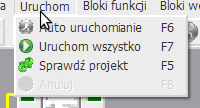
\includegraphics[scale=0.5]{uruchom}
 \caption{Uruchom}
 \label{fig:Run}
\end{figure}
\begin{description}
\item [Auto uruchamianie] Opcja typu ``toogle'', pozwala na włączanie trybu auto-uruchamiania projektu.
\item [Uruchom wszystko] Opcja uruchamia projekt, przetważane są wszystkie mozliwe bloczki nie uwzględniając ostatnie uruchomienia.
\item [Spradź projekt] Opcja wymusza przeprowadzenie sprawdzenia wszystkich bloczków.
\item [Anuluj] Opcja przerywa uruchamianie projektu.
\end{description}

\subsubsection{Menu dynamicznych bloczków}
W tym miejscu znajdują się menu ładowane z plików koniguracyjnych, każda opcja pozwala na dodanie ściśle powiązanego z nia bloczka, ilośc tych menu i struktura nie jest ściśle określona.

\subsubsection{Pomoc}
\begin{description}
\item [Instrukcja użytkownika] Wyświetla ten plik.
\item [Dokumentacja techniczna] Wyświetla dokument zawierający informacje przydatne dla developerów lub osób które by chiały wprowadzic zmiany do projektu.
\item [O autorach] Wyświetla okno pokazujące informacje o autorach programu jak i ich zanagażowanie.
\item [O programie] Wyświetla okno pokazujące krótkie informacje o programie.
\end{description}

\subsection{Toolbar}
Toolbar jest to szereg przyciskow widocznych zaraz pod menu. Ich funkcje są takie same jak ich odpowiednikom w menu a kolejść jest nastepująca:
\begin{figure}[h]
 \centering
 
\includegraphics[scale=0.5]{toolbar}
 \caption{Toolbar}
 \label{fig:Toolbar}
\end{figure}

\begin{itemize}
 \item Nowy projekt
 \item Otwórz projekt
 \item \textit{Separator}
 \item Zapisz projekt
 \item Zapisz projekt jako
 \item \textit{Separator}
 \item Zamknij projekt
 \item \textit{Separator}
 \item Zaznacz wszystkie bloki
 \item Duplikuj wszystkie bloki
 \item Usuń zaznaczony blok lub połączenie
 \item Zresetuj połączenie
 \item \textit{Separator}
 \item Auto-uruchamianie
 \item Uruchom
 \item Sprawdź projekt
 \item Anuluj
 \item \textit{Separator}
 \item Przycisk pozwalający na dodanie ostatnio dodawanego bloczka
 \item Przycisk pozwalający na dodanie drugiego w kolejności ostatnio dodawanego bloczka
 \item Przycisk pozwalający na dodanie trzeciego w kolejności ostatnio dodawanego bloczka
 \item Przycisk pozwalający na dodanie czwartego w kolejności ostatnio dodawanego bloczka
 \item Przycisk pozwalający na dodanie piątego w kolejności ostatnio dodawanego bloczka
 \item \textit{Separator}
 \item Instrukcja użytkownika
 \item O autorach
 \item O programie
\end{itemize}

\subsection{Strefa projektu}
Przestrzeń w której zarządzamy bloczkami/połaczeniami. Tutaj możemy zmieniać położenie bloczków oraz ich połączenia. Dokładny opis bloczków znajduję sie w sekcji Zarządzanie projektem.
Podstawowe operacje wykonywane na bloczkach to:
\begin{figure}[h]
 \centering
 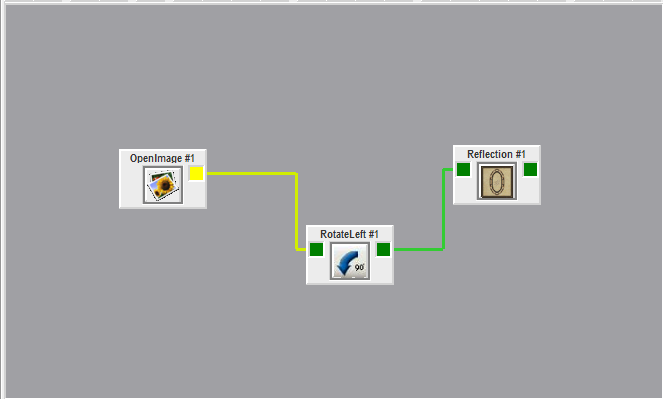
\includegraphics[scale=0.5]{strefaprojektu}
 \caption{Strefa Projektu}
 \label{fig:Interface}
\end{figure}
\begin{itemize}
 \item Przesuwanie
 \item Usuwanie
 \item blabla
\end{itemize}

\subsection{System logów}
System wyświetlania logów jest podzielony na 3 strefy:
\begin{figure}[h]
 \centering
 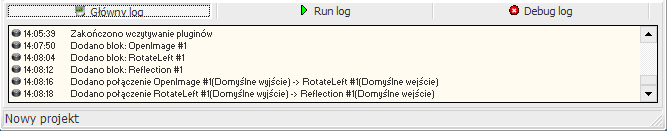
\includegraphics[scale=0.5]{systemlogow}
 \caption{System Logów} 
 \label{fig:systemlogow}
\end{figure}
\begin{description}
 \item[Główny log] Wyświetlane są tu wszystkie logi oprócz Debug, Run log
 \item[Run log] Wyświetlane są tu informacje natemat przetważanych bloczków, Logi te są usuwane przed każdym uruchomieniem projektu.
 \item[Debug log] Wyświetlane sa tu wszystkie możliwe logi.
 \end{description}
Kolory komunikatów:
\begin{description}
 \item[Czarny] - informacja
 \item[Niebieski] - debug
 \item[Zólty] - ostrzeżenie
 \item[Czerwony] - błąd
 \item[Zielony] - sukces
 \end{description}
Klikając prawym przyciskiem na liście logów pokaże się menu pozwalające na wyczyszczenia aktualnych logów lub zapisanie ich do pliku.
\subsection{Pasek status}
Aktualnie jedyną funkcja paska statusu jest wyświetlanie aktualnie otwartego projektu.
\begin{figure}[h]
 \centering
 
\includegraphics[scale=0.5]{status}
 \caption{Status}
 \label{fig:Status}
\end{figure}
\section{Skróty klawiatury}
\begin{description}
 \item[Ctrl+N] - Nowy projeky
 \item[Ctrl+O] - Otórz projekt
 \item[Ctrl+S] - Zapisz projekt
 \item[Shift+Ctrl+S] - Zapisz projekt jako
 \item[Ctrl+C] - Zamknij projekt
 \item[Ctrl+X] - Zakończ
 \item[Ctrl+A] - Zaznacz wszystkie bloki
 \item[Ctrl+U] - Odznacz wszystkie bloki
 \item[Ctrl+I] - Odwróć zaznaczenie bloków
 \item[Ctrl+D] - Duplikuj zaznaczone bloki
 \item[Shift+Del] - Usuń wszystkie bloki
 \item[Alt+D] - Usuń zaznaczone bloki
 \item[Ctrl+E] - Odznacz zaznaczone połączenie
 \item[Ctrl+Del] - Usuń wszystkie połączenia
 \item[Shift+D] - Usuń zaznaczone połączenie
 \item[Shift+R] - Zresetuj wszystkie połaczenia
 \item[Ctrl+R] - Zresetuj zaznaczone połączenie
 \item[Del] - Usuń zaznaczone bloki lub połączenie
 \end{description}
\section{Zarządzanie projektem}
\subsection{Bloczki}
Pojedynczy blok reprezentuję operację na obrazie (np. Binaryzacja,Wczytywanie,Zapisywanie). Na każdym bloku widnieje jego nazwa i numer.
\begin{enumerate}
 \item Kliknięcie lewym przyciskiem myszy na bloku zaznacza go ale odznacza inne bloki
 \item Klikniecie lewym przyciskiem myszy na bloku trzymając wcisniety klawisz Ctrl zaznacza blok, ale nie odznacza innych bloków
 \item Nacisniecie prawego przycisku myszy zezwala na przenoszenie bloczka.
 \item Nacisnięcie prawego przycisku myszy tzrymając wciśnięty klawisz Ctrl zezwala na przenoszenie wszystkich zaznacoznych bloków + blok na którym sie klikneło.
 \item Nacisniecie lewego przycisku myszy na bloku trzymając wciśniety klawisz Shift zaznacza blok i zezwala na jego przenoszenie.
 \item Nacisniecie lewego przycisku myszy na bloku trzymając wciśniety klawisz Shift+Ctrl zaznacza blok i zezwala na przenoszenie wszystkich zaznaczonych bloków.
\end{enumerate}

\subsubsection{Wejścia}
Z lewej strony bloczku znajdują się wejścia, które są tworzone dynamicznie. Bloczek taki jak wczytywanie obrazu nie posiada żadnego wejścia gdyż nie przetwarza on żadnych danych, plik do wczytania zostaje podany w konfiguracji. Większość bloczków posiada tylko jedno wejście. Jednakże mogą istnieć bloczki które będą wymagały podania więcej niż jednego wejścia (na przykład dodawanie obrazów). Jest także możliwość że w bloczku może się pojawić nie tylko wiele wejśc ale również i całkowicie innych typów.
Stan wejścia jest opisywany poprzez kolor połączenia a także poprzez opis (który jest wyświetlany po najechaniu na wejście).
\begin{figure}[h]
 \centering
 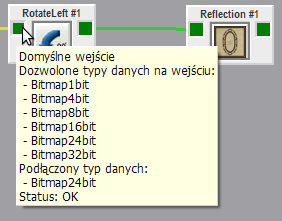
\includegraphics[scale=0.5]{wejscia}
 \caption{Wejscia}
 \label{fig:Input}
\end{figure}
Kliknięcie lewym przyciskiem myszy na wejściu ``wybiera'' wejście.
Kliknięcie prawym przyciskiem myszy na wejściu otwiera okno histori dla danego bloku z zaznaczeniem wejścia.
\subsubsection{Wyjścia}
Wynik przetwarzania jest symbolizowany z prawej strony bloczka jako wyjscie. Ilośc wyjśc jak i ich typ zależy od bloczka.
\begin{figure}[h]
 \centering
 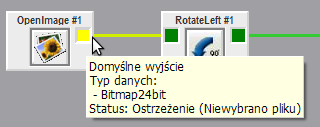
\includegraphics[scale=0.5]{wyjscia}
 \caption{Wyjscia}
 \label{fig:Output}
\end{figure}
Kliknięcie lewym przyciskiem myszy na wyjściu ``wybiera'' wyjściu.
Kliknięcie prawym przyciskiem myszy na wyjściu otwiera okno histori dla danego bloku z zaznaczeniem wyjścia.
\subsubsection{Przycisk konfiguracyjny}
Po kliknięciu na przycisk konfiguracji pojawia się okno opcji dotyczących przeprowadzenia danej operacji, lecz nie danych które powinny zostać przesłane do bloku poprzez wejście. Nie każdy bloczek musi posiadac konfiguracje.
\begin{figure}[h]
 \centering
 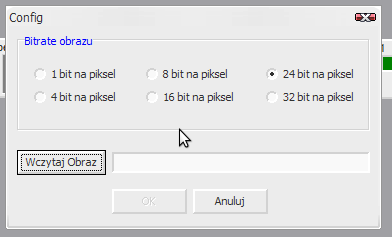
\includegraphics[scale=0.5]{config}
 \caption{Konfiguracja}
 \label{fig:config}
\end{figure} 
\subsubsection{Status}
Stan w jakim znajduje sie bloczek jest w tym samym czasie symbolizowany na kilka sposobów. Kolor obramowania wokół przycisku konfiguracyjnego symbolizuje stan bloczka.
\begin{description}
 \item[Szary] Bloczek nie był jeszcze uruchamiany
 \item[Zielony] Bloczek został uruchamiany poprawnie
 \item[Zółty] Bloczek nie został uruchomiony ze względu na brak wymaganych danych.
 \item[Czerwony] Wystapił błąd podczas uruchamiania bloczka
 \end{description}
\subsection{Połączenia}
Połączenia między blokami definiują sposob przepływu danych miedzy blokami.
\begin{itemize}
 \item System zezwala tylko na podłączenie jednego połaczenia do pojedyńczego wejścia.
 \item System nie zezwala na połączenia cykliczne.
 \item Kliknięcie prawym przyciskiem na połączeniu resetuje jego modyfikacje pozycji i rozmiaru.
 \item Kliknięcie lewym przyciskiem na połączeniu zaznacza go.
 \item Przytrzymanie lewego klawisza myszy na połączeniu pozwala na dostosowanie wymiarów i kształtu połączenia do własnych potrzeb.
\end{itemize}

\subsection{Historia}
Po każdym poprawnym uruchomieniu dla każdego bloczka jest zapamiętywana historia. W historii może być zapsianych maksymalnie 10 ostatnich uruchomień 
\subsection{Eksport/Import}
\subsection{Uruchamianie}
\section{Podsumowane}

\end{document}
